% End-to-end monitoring pipeline of the Wasserstein Drift Detector.
% Build: pdflatex pipeline.tex  ->  pipeline.pdf (included by main.tex).
\documentclass[tikz,border=2pt]{standalone}
\usepackage{amsmath,amssymb}
\usetikzlibrary{arrows.meta,calc,fit,backgrounds,decorations.pathreplacing}

\definecolor{dataC}{HTML}{0072B2}
\definecolor{detC}{HTML}{555555}
\definecolor{alarmC}{HTML}{D55E00}
\definecolor{calC}{HTML}{009E73}

\begin{document}
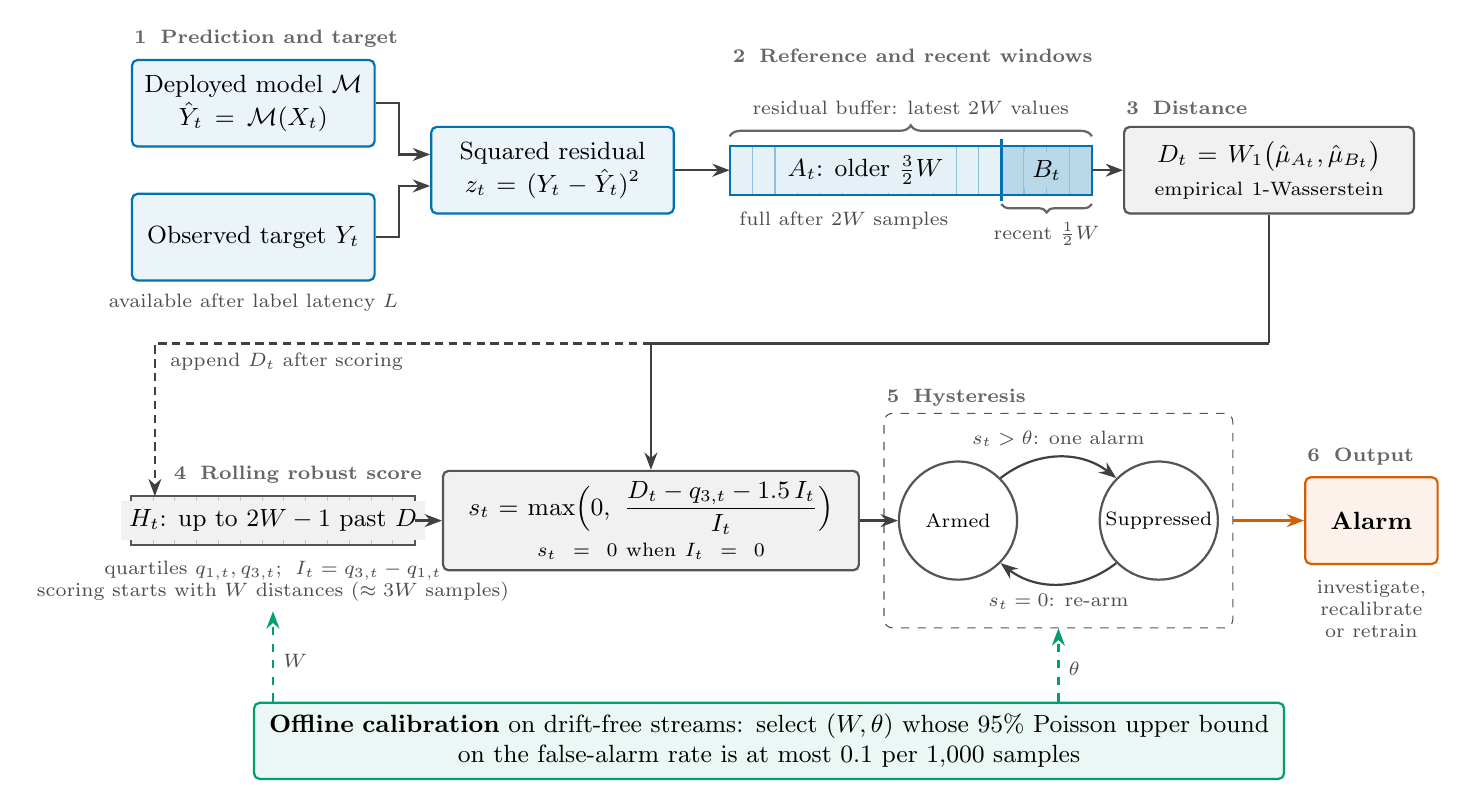
\begin{tikzpicture}[
  font=\small,
  >={Stealth[length=2.2mm]},
  flow/.style={->,thick,draw=black!75},
  box/.style={draw=#1,fill=#1!8,rounded corners=2pt,align=center,inner sep=4pt,minimum height=11mm,thick},
  box/.default=detC,
  stage/.style={font=\scriptsize\bfseries,text=black!60,anchor=south west,inner sep=1pt},
  note/.style={font=\scriptsize,text=black!70,align=center},
  state/.style={circle,draw=detC,fill=white,thick,minimum size=15mm,inner sep=0pt,align=center,font=\scriptsize},
]

% ------------------------------------------------------------------ row 1
\node[box=dataC,text width=28mm] (model) at (1.55,0.85)
  {Deployed model $\mathcal M$\\[1pt]$\hat Y_t=\mathcal M(X_t)$};
\node[box=dataC,text width=28mm] (target) at (1.55,-0.85)
  {Observed target $Y_t$};
\node[box=dataC,text width=28mm] (resid) at (5.35,0)
  {Squared residual\\[1pt]$z_t=(Y_t-\hat Y_t)^2$};

\draw[flow] (model.east) -- ++(0.3,0) |- ([yshift=2mm]resid.west);
\draw[flow] (target.east) -- ++(0.3,0) |- ([yshift=-2mm]resid.west);
\node[note,anchor=north] at ([yshift=-1pt]target.south) {available after label latency $L$};
\node[stage] at ([yshift=1mm]model.north west) {1\;\;Prediction and target};

% residual buffer: latest 2W residuals; older 3W/2 = A_t, recent W/2 = B_t
\def\bx{7.6}\def\bw{4.6}\def\bh{0.62}
\pgfmathsetmacro{\bsplit}{\bx+0.75*\bw}
\pgfmathsetmacro{\bend}{\bx+\bw}
\fill[dataC!10] (\bx,-\bh/2) rectangle (\bsplit,\bh/2);
\fill[dataC!28] (\bsplit,-\bh/2) rectangle (\bend,\bh/2);
\foreach \i in {1,...,15} {\draw[dataC!45] ({\bx+\i*\bw/16},-\bh/2) -- ({\bx+\i*\bw/16},\bh/2);}
\draw[dataC,thick] (\bx,-\bh/2) rectangle (\bend,\bh/2);
\draw[dataC,very thick] (\bsplit,-\bh/2-0.08) -- (\bsplit,\bh/2+0.08);
\node at ({(\bx+\bsplit)/2},0) {\colorbox{dataC!10}{$A_t$: older $\tfrac32W$}};
\node at ({(\bsplit+\bend)/2},0) {\colorbox{dataC!28}{$B_t$}};
\draw[decorate,decoration={brace,amplitude=4pt},thick,black!60]
  (\bx,\bh/2+0.12) -- (\bend,\bh/2+0.12)
  node[midway,above=4pt,note] {residual buffer: latest $2W$ values};
\draw[decorate,decoration={brace,amplitude=3pt,mirror},thick,black!60]
  (\bsplit,-\bh/2-0.12) -- (\bend,-\bh/2-0.12)
  node[midway,below=3pt,note] {recent $\tfrac12W$};
\node[note,anchor=north west] at (\bx,-\bh/2-0.1) {full after $2W$ samples};
\node[stage] at (\bx,1.33) {2\;\;Reference and recent windows};
\draw[flow] (resid.east) -- (\bx,0);

\node[box,text width=34mm] (dist) at (14.45,0)
  {$D_t=W_1\big(\hat\mu_{A_t},\hat\mu_{B_t}\big)$\\[1pt]{\scriptsize empirical $1$-Wasserstein}};
\node[stage] at ([yshift=1mm]dist.north west) {3\;\;Distance};
\draw[flow] (\bend,0) -- (dist.west);

% ------------------------------------------------------------------ row 2
\def\ry{-4.45}
% rolling distance history
\def\hx{0.0}\def\hw{3.6}
\fill[detC!8] (\hx,\ry-\bh/2) rectangle ({\hx+\hw},\ry+\bh/2);
\foreach \i in {1,...,12} {\draw[detC!35] ({\hx+\i*\hw/13},\ry-\bh/2) -- ({\hx+\i*\hw/13},\ry+\bh/2);}
\draw[detC,thick] (\hx,\ry-\bh/2) rectangle ({\hx+\hw},\ry+\bh/2);
\node at ({\hx+\hw/2},\ry) {\colorbox{detC!8}{$H_t$: up to $2W-1$ past $D$}};
\coordinate (histN) at ({\hx+0.3},\ry+\bh/2);
\coordinate (histE) at ({\hx+\hw},\ry);
\node[note,anchor=north] (qnote) at ({\hx+\hw/2},\ry-\bh/2-0.08)
  {quartiles $q_{1,t},q_{3,t}$;\; $I_t=q_{3,t}-q_{1,t}$\\scoring starts with $W$ distances ($\approx3W$ samples)};
\node[stage] at (\hx+0.5,\ry+\bh/2+0.12) {4\;\;Rolling robust score};

\node[box,text width=50mm] (score) at (6.6,\ry)
  {$s_t=\max\!\Big(0,\;\dfrac{D_t-q_{3,t}-1.5\,I_t}{I_t}\Big)$\\[2pt]{\scriptsize $s_t=0$ when $I_t=0$}};
\draw[flow] (histE) -- (score.west);

% hysteresis state machine
\node[state] (armed) at (10.5,\ry) {Armed};
\node[state] (supp)  at (13.05,\ry) {Suppressed};
\draw[flow] (armed.north east) to[bend left=38]
  node[midway,above,note] {$s_t>\theta$: one alarm} (supp.north west);
\draw[flow] (supp.south west) to[bend left=38]
  node[midway,below,note] {$s_t=0$: re-arm} (armed.south east);
\begin{scope}[on background layer]
  \node[draw=detC,dashed,rounded corners=3pt,fit=(armed)(supp),inner xsep=5pt,inner ysep=17pt] (hyst) {};
\end{scope}
\node[stage] at ([yshift=1pt]hyst.north west) {5\;\;Hysteresis};
\draw[flow] (score.east) -- (armed.west);

\node[box=alarmC,text width=14mm,font=\small\bfseries] (alarm) at (15.75,\ry) {Alarm};
\node[note,anchor=north] at ([yshift=-2pt]alarm.south) {investigate,\\recalibrate\\or retrain};
\node[stage] at ([yshift=1mm]alarm.north west) {6\;\;Output};
\draw[flow,draw=alarmC] (hyst.east |- supp.east) -- (alarm.west);

% distance bus: D_t is scored, then appended to the history
\def\busy{-2.2}
\draw[thick,black!75] (dist.south) -- (dist.south |- 0,\busy);
\draw[flow] (dist.south |- 0,\busy) -| (score.north);
\draw[flow,densely dashed] (score.north |- 0,\busy) -| (histN);
\node[note,anchor=north west] at ([xshift=2pt]histN |- 0,\busy) {append $D_t$ after scoring};

% ------------------------------------------------------------------ calibration
\node[box=calC,text width=128mm,minimum height=9mm,anchor=north] (calib) at (8.1,-6.75)
  {\textbf{Offline calibration} on drift-free streams: select $(W,\theta)$ whose 95\% Poisson upper bound\\on the false-alarm rate is at most $0.1$ per $1{,}000$ samples};
\draw[->,thick,dashed,draw=calC] (calib.north -| qnote.south) -- node[pos=0.45,right,note] {$W$} (qnote.south);
\draw[->,thick,dashed,draw=calC] (calib.north -| hyst.south) -- node[pos=0.45,right,note] {$\theta$} (hyst.south);

\end{tikzpicture}
\end{document}
